%Przykładowy plik ułatwiający złożenie projektu dyplomowego inżynierskiego.
%UWAGA: Generowany napis na stronie tytułowej o treści PROJEKT DYPLOMOWY INŻYNIERSKI został zaproponowany przeze mnie i nie jest, póki co, potwierdzony przez władze wydziału. Przed ostatecznym oddaniem tak złożonej pracy należy upewnić się jaka powinna być treść tego napisu. W momencie gdy uzyskam informację na temat treści tego napisu, dokonam niezbędnych zmian w źródłach.

\documentclass[eng,printmode]{mgr}
%opcje klasy dokumentu mgr.cls zostały opisane w dołączonej instrukcji

%poniżej deklaracje użycia pakietów, usunąć to co jest niepotrzebne
\usepackage{polski} %przydatne podczas składania dokumentów w j. polskim
%\usepackage[polish]{babel}%alternatywnie do pakietu polski, wybrać jeden z nich
\usepackage[utf8]{inputenc} %kodowanie znakĂłw, zaleĹĽne od systemu
\usepackage[T1]{fontenc} %poprawne składanie polskich czcionek

%pakiety do grafiki
\usepackage{graphicx}
\usepackage{subfigure}
\usepackage{psfrag}
\usepackage[polish]{babel}
\usepackage[utf8]{inputenc}
\usepackage{lmodern}
\selectlanguage{polish}
%pakiety dodające dużo dodatkowych poleceń matematycznych
\usepackage{amsmath}
\usepackage{amsfonts}

%pakiety wspomagające i poprawiające składanie tabel
\usepackage{supertabular}
\usepackage{array}
\usepackage{tabularx}
\usepackage{hhline}

%pakiet wypisujący na marginesie etykiety równań i rysunków zdefiniowanych przez \label{}, chcąc wygenerować finalną wersję dokumentu wystarczy usunąć poniższą linię
\usepackage{showlabels}

%definicje własnych poleceń
\newcommand{\R}{I\!\!R} %symbol liczb rzeczywistych, działa tylko w trybie matematycznym
\newtheorem{theorem}{Twierdzenie}[section] %nowe otoczenie do składania twierdzeń

%dane do złożenia strony tytułowej
\title{Wyznaczanie kierunku przylotu sygnału akustycznego z zastosowaniem systemu mikrofonów}
\engtitle{Determination of the direction of acoustic signal arrival using a microphone system}
\author{Paweł Rachwalski}
\supervisor{dr inż. Bogdan Kreczmer. PWr, I-6}
%\guardian{dr hab. inż. Imię Nazwisko Prof. PWr, I-6} %nie używać jeśli opiekun jest tą samą osobą co prowadzący pracę

%\date{2008} %standardowo u dołu strony tytułowej umieszczany jest bieżący rok, to polecenie pozwala wstawić dowolny rok

%poniżej jest lista kierunków i specjalności na wydziale elektroniki, należy wybrać właściwe lub dopisać jeśli nie ma odpowiednich
\field{Automatyka i Robotyka (AIR)}
\specialisation{Robotyka (ARR)}
%\specialisation{Komputerowe sieci sterowania (ARK)}
%\specialisation{Systemy informatyczne w automatyce (ASI)}
%\specialisation{Komputerowe systemy zarzÄ…dzania \\procesami produkcyjnymi (ARS)}
%\field{Elektronika i telekomunikacja (EIT)}
%\specialisation{Akustyka (ETA)}
%\specialisation{Aparatura elektroniczna (EAE)}
%\specialisation{Elektroniczne i komputerowe \\systemy automatyki (ESA)}
%\specialisation{Zastosowania inĹĽynierii komputerowej \\w technice (EZI)}
%\specialisation{Inżynieria dźwięku (EID)}
%\specialisation{Elektronika stosowana \\i optokomunikacja (TEO)}
%\specialisation{Telekomunikacyjne sieci szerokopasmowe (TSS)}
%\specialisation{Teleinformatyczne sieci mobilne (TSM)}
%\specialisation{Sygnały w telekomunikacji cyfrowej (TSC)}
%\specialisation{Teleinformatyczne systemy rozsiewcze (TSR)}
%\field{Informatyka (INF)}
%\specialisation{Systemy informatyki w medycynie \\i technice (IMT)}
%\specialisation{InĹĽynieria systemĂłw informatycznych (INS)}
%\specialisation{InĹĽynieria internetowa (INT)}
%\specialisation{Systemy i sieci komputerowe (ISK)}
%\field{Teleinformatyka (TIN)}
%\specialisation{Teleinformatyka (TIN)}

%tutaj zaczyna się właściwa treść dokumentu
\begin{document}
\bibliographystyle{plabbrv} %tylko gdy uĹĽywamy BibTeXa, ustawia polski styl bibliografii

\maketitle %polecenie generujące stronę tytułową
\dedication{6cm}{Pracę tę dedykuję rodzicom, w podziękowaniu za wsparcie i wiarę w moje możliwości}

\tableofcontents %spis treści

%poniżej znajduje się przykładowa treść dalszej części dokumentu, zainteresowanych zachęcam do rozszyfrowania frazy "Lorem ipsum" :)
\chapter{Wstęp}
Wstępwstepepepepepepepepeppeepep

\chapter{Analiza problemu}
Analaliza

\section{Nulla quis enim ut erat rutrum feugiat}
Nulla quis enim ut erat rutrum feugiat. Suspendisse lacinia tempor mi. Vestibulum nec lacus sed est rutrum cursus. Cras ultrices est eget pede. Sed ullamcorper ultrices tellus. Nulla lectus. Nunc consectetuer, quam quis sagittis vulputate, dui leo molestie augue, a commodo tellus tortor a turpis. Nam et ipsum. Ut placerat aliquet enim. Suspendisse potenti. Etiam volutpat tortor in mauris. Praesent dapibus congue arcu. 

In hac habitasse platea dictumst. In pulvinar, leo sit amet placerat laoreet, metus metus porttitor mi, vitae nonummy nisi sem eget sapien. In velit velit, pellentesque ac, luctus vel, ornare malesuada, leo. Nunc quis sapien. Vivamus risus justo, faucibus sit amet, varius et, bibendum at, tortor. Quisque in arcu sit amet velit faucibus dignissim. Phasellus dapibus ante non risus. Nunc magna turpis, vehicula quis, egestas sit amet, accumsan sit amet, lorem. Curabitur eu felis in ligula elementum luctus. Aenean porttitor dui sed tellus ultrices vestibulum. Morbi neque. 



\begin{itemize}
\item Mauris nonummy lorem at orci.
\item Donec accumsan aliquam libero.
\item Donec fringilla ultricies diam.
\item Nulla venenatis est non ligula.
\item Morbi in mi convallis dolor accumsan egestas.
\item Sed euismod nibh in nulla.
\item Sed rhoncus lorem at lectus.
\item Pellentesque fermentum rutrum dui.
\end{itemize}

Proin euismod. Curabitur adipiscing ipsum ac augue. Maecenas hendrerit tortor non velit suscipit laoreet. Aenean tempus. Nunc convallis. Aenean sed erat. Etiam massa nulla, interdum pretium, faucibus nec, sollicitudin vitae, lorem. Quisque vulputate cursus pede. Phasellus enim ipsum, lacinia vel, sodales ac, faucibus et, tortor. Aliquam hendrerit. Aliquam erat volutpat. Quisque dui lorem, placerat eu, commodo et, condimentum sed, nibh. Nulla eu orci in nibh pretium tincidunt. Pellentesque mi massa, fringilla eu, vehicula consectetuer, sodales a, nisi. 

Vivamus ut risus in quam porttitor venenatis. Phasellus iaculis enim id pede. Etiam aliquam vehicula nibh. Cras congue dui. Mauris velit. Morbi eu magna nec ligula laoreet cursus. In pulvinar dui a urna. Morbi commodo. Cras non tortor in lorem fringilla volutpat. Duis et turpis. Quisque sit amet massa. Aliquam et metus eget lectus venenatis egestas. Nulla facilisi. Nulla tellus arcu, mollis eget, nonummy non, sollicitudin id, tellus. 

Quisque pretium eleifend turpis. Nulla ut pede gravida ante iaculis convallis. Quisque luctus, eros a varius rutrum, ligula ligula venenatis nisi, ut nonummy nisl ipsum vitae est. Etiam mauris risus, blandit ac, placerat id, varius consectetuer, pede. Fusce cursus diam a arcu. Pellentesque luctus turpis. Sed tortor. Sed eget arcu. Maecenas sed leo eget nunc fringilla ornare. Aenean purus justo, tristique eu, iaculis a, convallis in, augue. Nam feugiat magna eu magna. 

Cum sociis natoque penatibus et magnis dis parturient montes, nascetur ridiculus mus. Donec justo diam, auctor vitae, consectetuer sed, aliquet non, lectus. Suspendisse id lectus. Integer fermentum metus non felis. Praesent dui augue, auctor non, congue sed, aliquam vel, quam. Fusce et ligula dignissim sapien congue scelerisque. Phasellus tincidunt. Aliquam tempus, leo sollicitudin commodo aliquam, neque nisl nonummy ante, ac tristique lacus odio nec libero. Cras nec nisl sed erat commodo eleifend. Vivamus tellus. Fusce nec nibh ut neque malesuada feugiat. Nam molestie volutpat lacus. Aliquam sollicitudin nunc at turpis. Maecenas lectus quam, aliquam nec, aliquet eget, porta non, massa. Duis viverra nonummy mauris.


\chapter{Specyfikacja projektu}
System składa się z trzech bloków:
\begin{itemize}
\item Blok matrycy czterech mikrofonów.
\item Blok odpowiedzialny za wygenerownie i filrację obwiedni sygnału. 
\item Blok mikrokontrolera.
\end{itemize}
\section{Matryca mikrofonów}
Projekt nie przewidywał budowy matrycy mikrofonów wraz z konstrukcją toru wzmocnienia, dlatego zdecydowano się na zakup gotowego rozwiązania. Na rynku dostępny jest duży wybór czujników mikrofonowych wraz z dedykowanymi układami wzmaczniaczy, dwa z nich zdawały się być najbardziej odpowiednie.\\
Pierwszym z nich jest detektor dźwięku SEN-14262 produkowany przez firmę SparkFun[Rysunek 3.1], posiada on mikrofon elektretowy o zakresie częstotliwości od 100Hz do 10000Hz. Za wzmocnienie sygnału mikrofonowego odpowiada układ LMV324 z możliwością zmiany wzmocnienia od 20dB do 60 dB, podstawowo wartość ta jest usatwiona na 40 dB. Cały moduł posiada aż trzy niezależne wyjścia:
\begin{itemize}
\item Audio - analogowy sygnał audio.
\item Envelope - analogowy sygnał umożliwiający pomiar amplitudy sygnału 
\item Gate - sygnał cyfrowy pozwalający na detekcje przekroczenia ustalonego poziomu amplitudy.
\end{itemize}

\begin{figure}

    \centering

  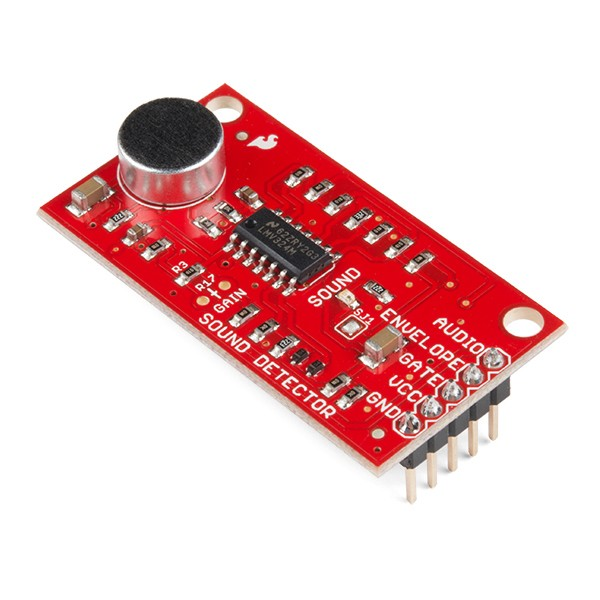
\includegraphics[width=0.33\textwidth, angle=0]{detektor1.jpg}

    \caption{SparkFun SEN-14262}

    

\end{figure}


 Drugie rozwiązanie to moduł czujnika dźwięku ze wzmaczniaczem MAX9814 produkowany przez firmę Adafruit[Rysunek 3.2], w jego skład wchodzi mikrofon elektretowy umożliwiający pomiary w zakresie 20Hz-20000Hz. Tor wzmacnienia czujnika jest oparty o układ MAX9814, który oferuje takie możliwości jak:
\begin{itemize}
\item AGC(Auto Gain Control) czyli automatycznie zmienne wzmocnienie zależne od poziomu natężenia sygnału wejściowego.
\item Zmienne maksymalne wzmocnienie sygnału 40dB-50dB-60dB. 
\item Ustawienie współczynnika Attack/Release 
\item sygnał wyjściowy na poziomie 2Vpp
\end{itemize}
\newpage
\begin{figure}

    \centering

  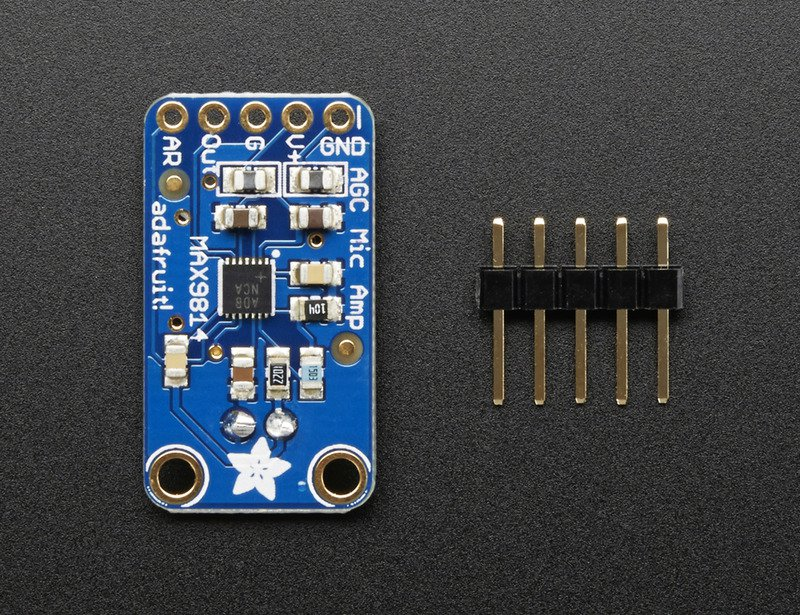
\includegraphics[width=0.33\textwidth, angle=0]{detektor2.jpg}

    \caption{Adafruit MAX9814}

    

\end{figure}

Ostatecznie wybrano rozwiązanie zaproponowane przez firmę Adafruit, ze względu na automatyczną kontrolę wzmocnienia, możliwość regulowania współczynnika Attack/Release oraz o wiele korzystaniejszą wartość współczynnika zawartości harmonicznych THD który w układzie MAX9814 dla częstotliwości 1kHz plasuje się na poziomie poniżej 0,1\%, dodatkowo MAX9814 posiada o wiele niższą gęstość szumów.
\section{Generator obwiedni}
Czujnik firmy Adafruit nie posiada wyjścia umożliwiającego pomiar amplitudy dlatego koniecznie jest skonstruowanie zewnętrznego układu odpowiadającego za generowanie obwiedni, rozwiąznie to podyktowane jest chęcią pominięcia złożonych obliczeń na mikrokontrolerze związanych z tranformatą Hilberta. Zastosowano prosty detektor obwiedni.
\begin{figure}

    \centering

  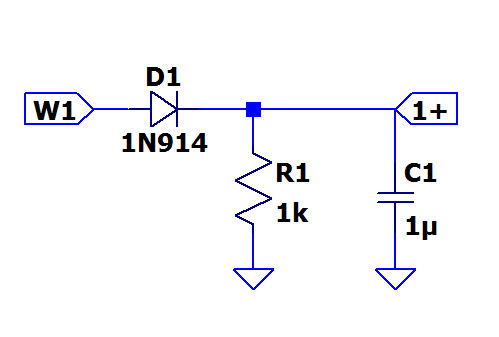
\includegraphics[width=0.6\textwidth, angle=0]{obwiednia.png}

    \caption{Schemat detektora obwiedni}


\end{figure}
\newpage
Dioda umożliwia przepływ prądu tylko jeśli zacisk wejściowy ma potencjał wyższy niż zacisk wyjściowy, kondensator gromadzi ładunek na zboczu narastającym następnie powoli uwalnia go przez rezystor gdy wzgórze opada co w efekcie pozwala uzyskać  filtr górnoprzepustowy. Do zbudowania układu użyto diody 1N914 ze względu na jej dużą szybkość przełączania, wysoką przewodność oraz niezawodność. 
\section{Mikrokontroler}
Kolejnym krokiem przetwarzania sygnału uzyskanego z matrycy mikrofonów jest jego spróbkowanie oraz konwersja do postaci cyfrowej, aby niepotrzebnie nie zwiększać ilości części w układzie elektronicznym zdecydowano się na zastosowanie przetwornika ADC który będzie jednym z peryferiów mikrokontrolera. Przy projektowaniu systemu brano pod uwagę głównie mikrokontrolery firmy STM32 ze względu na:
\begin{itemize}
\item Generator szkieletu projektu CubeMX który przyśpiesza pracę związane z konfiguracją.
\item Wiele darmowych narzędzi oraz przejrzyste IDE SW4.
\item Biblioteke HAL ułatwiajacą pracę z peryferiami.
\item Prostote debuggowania przy pomocy STM studio.
\end{itemize} 
Poszukiwania zawężono do mikrokontrolerów z rodziny F4, ponieważ są one oparte na rdzeniu CortexM4 pozwalającym na szybką pracę z jednostkami zmiennoprzecinkowymi oraz szybkie obliczenia dzięki wysokiemu taktowaniu rdzenia. Finalnie wybór padł na jednostkę STM32F446RET6, jej zalety szczególnie przydatne przy danym projekcie to:
\begin{itemize}
\item Częstotliwość taktowania do 180Mhz.
\item Trzy przetworniki ADC o rozdzielczości 12 bitów.
\item 16- strumieniowy kontroler DMA.
\item 6 interfejsów UART, które pozwolą na jednoczesne monitorowanie każdego z mikrofonów przy przeprowadzaniu testów.
\item 128kB pamięci RAM.
\end{itemize} 
% \appendix tworzy dodatek

\addcontentsline{toc}{chapter}{\bibname} %utworzenie w spisie treści pozycji Literatura
\bibliography{bibliografia} % wstawia bibliografię korzystając z pliku bibliografia.bib - dotyczy BibTeXa, jeżeli nie korzystamy z BibTeXa należy użyć otoczenia thebibliography

%opcjonalnie może się tu pojawić spis rysunków i tabel
% \listoffigures
% \listoftables
\end{document}

